\documentclass[12pt]{article}
 
\usepackage[margin=.95in]{geometry} 
\usepackage{amsmath,amsthm,amssymb, graphicx, multicol, array}
 
\newcommand{\N}{\mathbb{N}}
\newcommand{\Z}{\mathbb{Z}}
 
\usepackage{enumitem}
\setlist{nosep}
\begin{document}
 
\title{Project Initial Report}
\author{Juliette Franqueville\\
}
\maketitle
\newpage
\section{Introduction}
The paper I have chosen for my project is ``Inferring causal impact using Bayesian Structural Time-Series Models'' from Google and by  Kay H. Brodersen, Fabian Galluser, Jim Koehler, Nicolas Remy and Steven L. Scott.

\section{Paper Summary}
This paper proposes a Bayesian method for inferring  the causal impact of a market intervention on a metric of interest. For example, the ``market intervention'' may be an advertising campaign, and the metric of interest may be number of sales. The causal impact of the market intervention is the difference between the results observed (with intervention) for the metric of interest and the results that would have been observed without the market intervention. In order to find this difference, the basic idea is to:\\
\begin{itemize}
    \item Fit a time-series model to the observed metric of interest prior to the market intervention
    \item Use the model to predict what the results for the metric of interest would have been without market intervention
    \item Compare the forecast to the metric of interest that was actually observed after the market intervention\\
    \end{itemize}  

There are three components that are useful in training the forecasting model for the unobserved data:\\

\begin{itemize}
    \item Observed data prior to the market intervention
    \item Data from a contemporaneous time series for which no market intervention happened  (for example, for another country where no advertising campaign was conducted) 
    \item Prior knowledge about the model parameters, given that the model is Bayesian\\
    \end{itemize}  

Figure \ref{fig:my_label} helps understand the concept. The $x$-axis is time and $y$-axis is metric of interest, such as sales. In (a), the date of the market intervention is shown by the vertical line. The red and green lines corresponding to $X1$ and $X2$ are two contemporaneous time series (i.e. could be from another country with no market intervention). The black line is the observed data. The blue dotted line is the forecast in the case of no market intervention, from the model run on observed data before intervention and $X1$ and $X2$. Plot (b) shows the difference between the prediction (i.e. no market intervention) and the observed data (with market intervention). Here, it seems that the market intervention increased the metric of interest.
    \begin{figure}[h!]
    \centering
    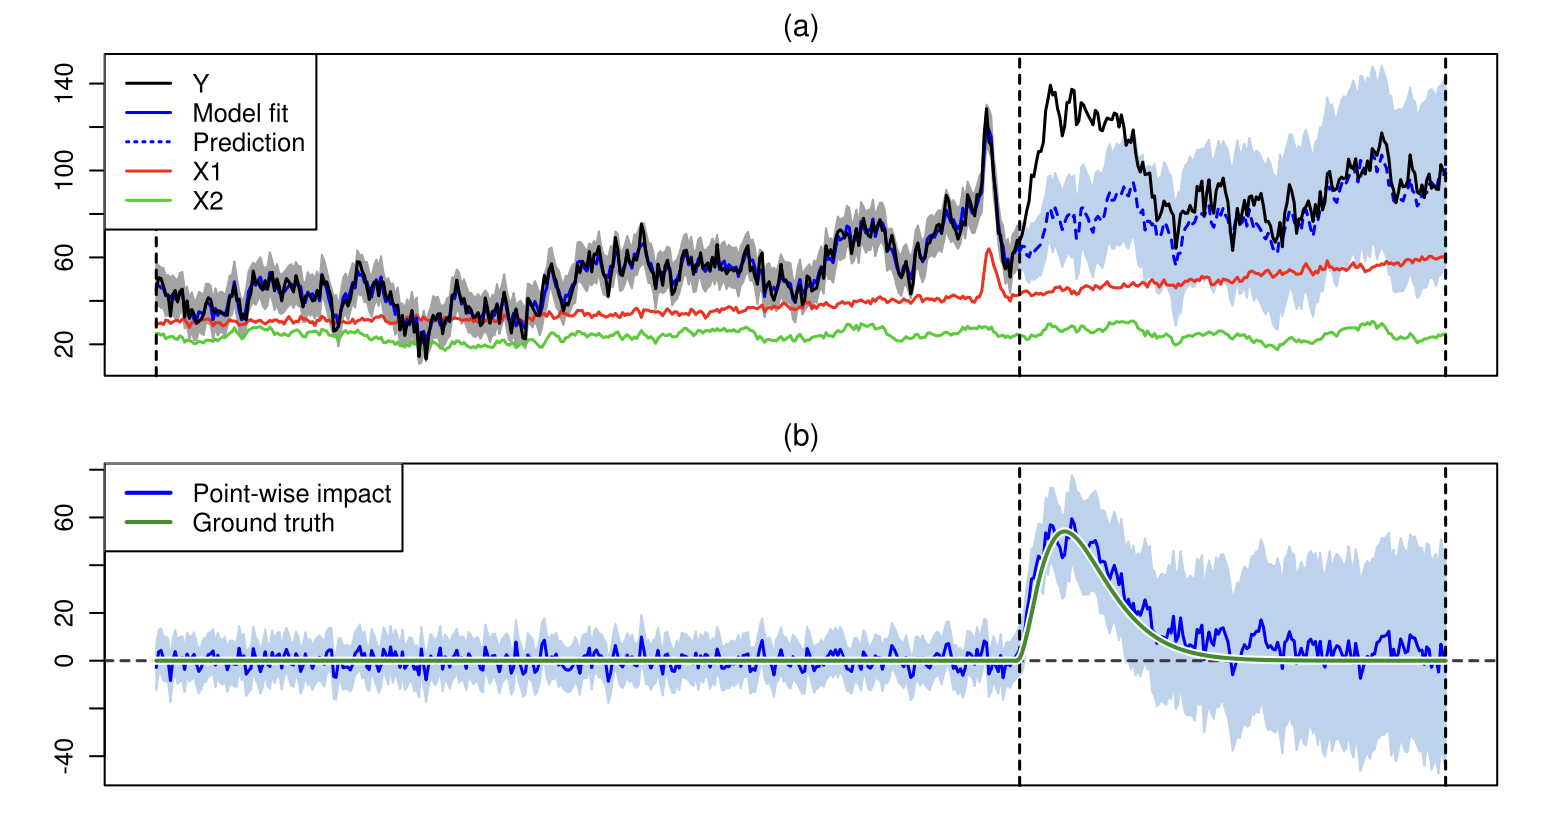
\includegraphics[scale=.4
    ]{figures/frompaper.png}
    \caption{Figures from paper.}
    \label{fig:my_label}
\end{figure}
An advantage of the Bayesian method is that it makes it easy to find posterior probability intervals as shown in (b).\\

Structural time-series models are a very broad class of models for time-series data. For example, they include all ARIMA models. There a four components of state associated with structural time-series models, described very briefly below:\\
\begin{itemize}
    \item \textbf{Local linear trend}, which assumes that  the mean and the slope of the trend follow random walks
    \item \textbf{Seasonality}, which captures seasonality in the data
    \item \textbf{Contemporaneous covariates with static coefficients,} which enable including contemporaneous time series using standard linear regression
    \item \textbf{Contemporaneous covariates with dynamic coefficients}, which is similar to the previous bullet point, but this time the regression coefficients follow a random walk\\
    \end{itemize}  
    
What makes the structural time-series model in this paper Bayesian is that all parameters are assigned prior probabilities. The posterior for the parameters can be simulated using a Gibbs sampler with a data-augmentation step (i.e. involving the introduction of an unobserved variable). The distribution of interest is however the posterior predictive distribution for the unobserved data (the blue dotted line and associated credible interval in Figure \ref{fig:my_label} (a), which can be obtained by sampling from the parameters' posterior distributions. Using the posterior predictive distribution, the data format shown in Figure \ref{fig:my_label} (b) can be obtained to help determine whether the marketing intervention was successful.\\

The paper features demonstrations of the model on simulated data and empirical data, which I intend to replicate.
\section{Progress}
So far, I have focused on:\\

\begin{itemize}
    \item Understanding simple time-series models to better understand how structural time-series models are structured
    \item Building the ``simulation'' dataset used in the first demonstration for the model
\end{itemize}


\end{document}